%-----------------------------------------
% Note: Use pdflatex to process this file.
%-----------------------------------------

\documentclass[11pt]{article}
%%\documentclass{book}
\usepackage{geometry}            % See geometry.pdf to learn the layout options. There are lots.
\usepackage{xspace}
\geometry{letterpaper}           % ... or a4paper or a5paper or ... 
%\geometry{landscape}            % Activate for for rotated page geometry
%\usepackage[parfill]{parskip}   % To begin paragraphs with an empty line rather than an indent
\usepackage{graphicx}
\usepackage{amssymb}
\usepackage{alltt}
%\usepackage{epstopdf}
%\DeclareGraphicsRule{.tif}{png}{.png}{`convert #1 `dirname #1`/`basename #1 .tif`.png}
\usepackage[T1]{fontenc}   % so _, <, and > print correctly in text.
\usepackage[strings]{underscore}    % to use "_" in text

\usepackage{hyperref}

%---------------------------------------------------------------------------------

\newcommand{\sref}[1]{$\S$\ref{#1}}
\newcommand{\syn}{\texttt{Synrad}\xspace}
\newcommand\ttcmd{\begingroup\catcode`\_=11 \catcode`\%=11 \dottcmd}
\newcommand\dottcmd[1]{\texttt{#1}\endgroup}
\newcommand{\Begineq}{\begin{equation}}
\newcommand{\Endeq}{\end{equation}}
\newcommand{\fig}[1]{Figure~\ref{#1}}
\newcommand{\vn}{\ttcmd}           
\newcommand{\Th}{$^{th}$\xspace}
\newcommand{\Newline}{\hfil \\}

\newenvironment{example}
  {\vspace{-3.0ex} \begin{alltt}}
  {\end{alltt} \vspace{-2.5ex}}

\newlength{\dPar}
\newlength{\ExBeg}
\newlength{\ExEnd}
\setlength{\dPar}{1.5ex}
\setlength{\ExBeg}{-\dPar}
\addtolength{\ExBeg}{-0.5ex}
\setlength{\ExEnd}{-\dPar}
\addtolength{\ExEnd}{-0.0ex}

%---------------------------------------------------------------------------------

\setlength{\textwidth}{6.25in}
\setlength{\hoffset}{0.0in}
\setlength{\oddsidemargin}{0.25in}
\setlength{\evensidemargin}{0.0in}
\setlength{\textheight}{8.5in}
\setlength{\topmargin}{0in}

\setlength{\parskip}{\dPar}
\setlength{\parindent}{0ex}

%---------------------------------------------------------------------------------

\title{\syn: Program for Calculating Synchrotron Radiation Power}
\author{}
\date{February 23, 2017}

\begin{document}
\maketitle

%------------------------------------------------------------------
\section{Introduction} 

\syn is a program for calculating the synchrotron radiation power
deposition on the beam chamber walls in a storage ring or
accelerator. \syn works by tracking X-rays from creation at the
beam to absorption at the chamber wall. The tracking is confined to
the horizontal plane. Reflections from the wall are not considered.
The vertical extent of the radiation stripe at the wall, important for
calculating the power deposition per unit area, is calculated using
the vertical emittance.

The chamber wall is specified in the horizontal plane by a set of
vertex points with a straight line between points. Exit and entrance
lines like x-ray beam lines or dumps can be modeled in \syn.
Shadowing of parts of the wall by other parts is taken into account in
the calculation.

Even though \syn only tracks photons in the horizontal plane, \syn
is able to handle lattices with non-horizontal bends. Radiation from
non-horizontal bends is included in the calculation. Obviously, if
this radiation is actually striking the top or bottom walls, \syn
will not give accurate results.

\syn output includes power deposition per longitudinal length, per
unit area on the beam center line, and photon flux. The beam orbit is
not constrained to be zero so calculations to see the affect of
varying the orbit are possible.

\syn is not to be confused with another program called Synrad3D.
The Synrad3D program uses Monte Carlo to generate photons along with a
full three dimensional chamber model along with a model for the
scattering the photons. The advantage of using \syn is that it is
quick and accurate since it does not rely on Monte Carlo methods.

\syn uses the Bmad subroutine library for relativistic
charged-particle simulations\cite{b:bmad} for some of the
calculations. 

%------------------------------------------------------------------
\section{Running \syn}
\label{s:run}

Syntax for invoking \syn:
\begin{example}
  <path-to-synrad-exe>/synrad \{-plot\} \{<master-input-file-name>\}
\end{example}
The \vn{<master-input-file-name>} optional argument is used to set the
master input file name. The default is ``\vn{synrad.in}''.

The optional \vn{-plot} option causes \syn to plot the vacuum
chamber walls. In this case, no synchrotron radiation calculations are
done.

%------------------------------------------------------------------

  \begin{figure}[tb]
  \begin{center}
  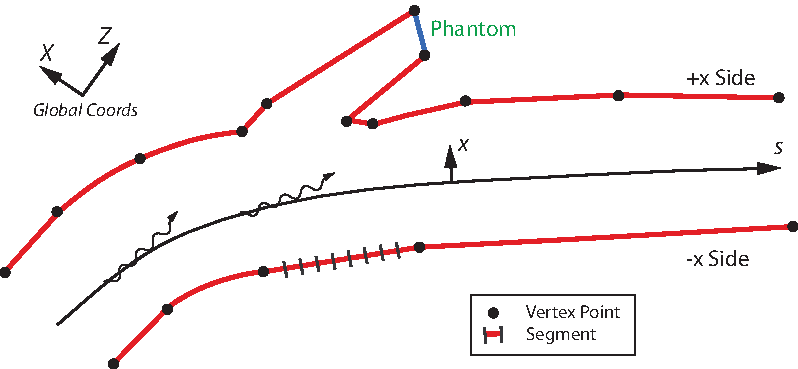
\includegraphics[width=5in]{wall.pdf}
  \caption{
The vacuum chamber wall has a $-x$ side and a $+x$ side. The wall is
defined by a number of vertex points (shown as circles) with straight
lines in $(x, s)$ between vertices. For the calculation, the straight
lines are divided into a number of roughly equal length short segments
as shown for a portion of the $-x$ side. Sections between vertex points
can also be declared as ``\vn{phantom}'' indicating that radiation 
striking such a section is not to be counted.
  }
  \label{f:wall}
  \end{center}
  \end{figure}

%------------------------------------------------------------------
\section{Vacuum Chamber Wall}
\label{s:wall}

\syn uses the Bmad local reference coordinates for specifying the
vacuum chamber wall (see the \vn{Coordinates} chapter in the Bmad
manual\cite{b:bmad}). The $s$-axis in this curvilinear coordinate
system is the longitudinal axis along the direction of the beam. If
there are no vertical bends, the $y$-axis is in the vertical
direction, and the $x$-axis is in the horizontal plane.

Since \syn is only tracking in the horizontal plane, the vacuum
chamber wall is divided into a ``positive $x$'' (``$+x$'') side and a
``negative $x$'' (``$-x$'') side as shown in Fig.~\ref{f:wall}. The
``$+x$'' section is defined as the wall on the positive $x$ side of
the centerline and vice versa. 

The $-x$ and $+x$ sides are specified by a number of vertex
points. Between vertex points, a straight line interpolation in $(x,
s)$ space is used to construct the wall. Since the coordinate system
is curvilinear, the actual shape of the wall in the global coordinate
system can be curved. For example, within a bend, a line of constant
$x$ in $(x, s)$ space will be mapped to the arc of a circle in the
$(X, Z)$ global coordinate system.

Sections between vertex points can also be declared as
``\vn{phantom}'' indicating that radiation striking such a section is
not to be counted. This is useful for simulating X-ray beam lines
where the X-rays traveling down the beam line does not contribute to
the power dissipated on the walls.

For the calculation, the lines between vertex points are broken up
into roughly equal length segments. While \syn tries to make
segments of equal size, since the distance between vertex points may
not be commensurate with the desired segment length, the actual
segment length can vary. For calculational purposes, segments are
treated as straight line segments in the global coordinate
system. That is, within a bend, only the ends of the segments will
truly lie on the straight line, in $(x, s)$ space, drawn between
vertices. Since the maximum segment length should be set to be much
smaller than any bend radius, the deviation caused in taking the
segments as straight in the global coordinate system should be
negligible.

Interpolation of the vacuum chamber wall between vertex points that
span a \vn{patch} element is problematical in that, in general, an
unbroken line in the $(x, s)$ coordinates will be discontinuous in the
global coordinates. This comes about since \vn{patch} elements can
introduce a discontinuity in the local reference coordinates. Since
this is not physical, \syn uses a different rule for interpolating
between vertex points that span a \vn{patch}. In such a case, linear
interpolation in the global coordinate system is used as shown in
Fig.~\ref{f:patch}. With this convention, the wall may be
discontinuous in $(x, s)$ space but this is not a problem since the
wall will be continuous in the global coordinate system.

%------------------------------------------------------------------

  \begin{figure}[tb]
  \begin{center}
  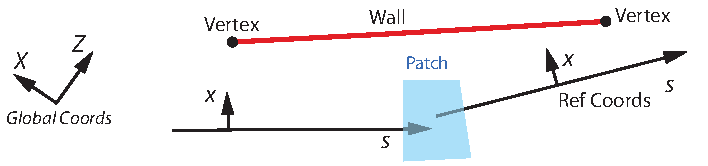
\includegraphics[width=5in]{patch.pdf}
  \caption{
The section of the vacuum chamber wall between two
vertices that span a patch element is constructed using
a straight line in the global coordinate system.
  }
  \label{f:patch}
  \end{center}
  \end{figure}

%------------------------------------------------------------------

In constructing the vacuum chamber wall, \syn will add vertex points
at the boundaries of bend magnets. This is generally transparent to
the user except it may result in segment lengths shifting slightly.
The $x$ values of the added points are interpolated using the $x$
values of the vertex points to either side, ignoring whether there are
any patch elements between the vertex points to either side. That is,
the interpolation is done in the curvalinear reference coordinate
system.

%------------------------------------------------------------------
\section{Simulation Technique} 

Photon generation is based on the standard synchrotron radiation
formulas, applicable for dipoles quadrupoles, and wigglers. The
radiation is assumed to be incoherent, so \syn cannot treat FEL
radiation. Since \syn only deals with the total emitted power (as
opposed to power emitted in a given energy bandwidth), \syn can
handle undulators.

Photons are generated roughly uniformly along the length of any
element where photons are produced. The generated photons are tracked
to the vacuum chamber wall. Tracking is confined to be in the
horizontal plane.  The power $P_b$ per unit angle bend of the particle
beam trajectory is\cite{b:sands}
\begin{equation}
  P_b \, \mbox{(W/radian)} = 14.3 \cdot 10^3  \, I_b \, \mbox{(Amps)} \, 
  [E_b \, \mbox{(eV)}]^4 \, [g \mbox{(1/m)}] 
\end{equation}
where $I_b$ is the beam current, $E_b$ is the beam energy, and $g =
1/R$ is the inverse of the bending radius. The power $P_{w1}$ per unit
wall length is then
\begin{equation}
  P_{w1} \, \mbox{(W/m)} = P_b \, \frac{\sin\theta_g}{L_p (m)}
\end{equation}
where $\theta_g$ is the grazing angle between the photon and the wall
and $L_p$ is the length the photon travels from generation to the wall.
The power $P_{w2}$ per unit area on the wall centerline is
\begin{equation}
  P_{w2} \, \mbox{(W/m$^2$)} = \frac{P_{w1}}{2 \, \pi \, \sigma_y}
\end{equation}
where $\sigma_y$ is the effective vertical sigma of the photon distribution at the wall 
\begin{equation}
  \sigma_y^2 = [\epsilon_y \, \beta_y] + [(\epsilon_y \, \gamma_y + 1 / \gamma^2) \, L_p^2]
\end{equation}
where $\beta_y$ and $\gamma_y$ are Twiss parameters, $\epsilon_y$ is
the vertical beam emittance, and $\gamma$ is the usual beam
relativistic factor. The first term in square brackets on the RHS of
the equation is the particle beam height and the second term is due to
the finite vertical opening angle of the photons.

Note: If the lattice is circular, photons leaving one end of the
lattice will be tracked through from the other end. That is, such
photons will be handled correctly. If the lattice is not circular,
photons reaching the ends of the lattice will be absorbed by the wall
there.

For a given element where radiation is produced, a set of $N$ photons
are generated and tracked. For wiggler radiation, the number of
photons produced per period of beam oscillation must be of order 10 or
more for an accurate calculation.  Each pair $(i, i+1)$ of photons, with
$i = 1, \ldots, N-1$, defines a section of the beam trajectory over which
radiation is produced.
The $i^{\mbox{th}}$ photon strikes
the wall at wall segment $W_i$. 
For each radiation section, the power incident on the wall segments between $W_i$
and $W_{i+1}$ is computed using interpolation. It is assumed that the
segment length is small enough so that power on a segment is
\begin{equation}
  P_s = l_s \, P_{s0}
\end{equation}
where $P_s$ is the integrated power over the segment, $l_s$ is the
segment length, and $P_{s0}$ is the power density at the center of the
segment. A check is made to see if any segments are shielded from the
photon flux by other parts of the wall. If so, the power on these
segments due to the radiation section is set to zero.

%------------------------------------------------------------------
\subsection{Fortran Namelist}
\label{s:namelist}

Fortran namelist syntax is used for parameter input by \syn. The
general form of a namelist is
\begin{example}
  &<namelist_name>
    <var1> = ...
    <var2> = ...
    ...
  /
\end{example}
The tag \vn{"\&<namelist_name>"} starts the namelist where
\vn{<namelist_name>} is the name of the namelist. The namelist ends
with the slash \vn{"/"} tag. Anything outside of this is
ignored. Within the namelist, anything after an exclamation mark
\vn{"!"} is ignored including the exclamation mark. \vn{<var1>},
\vn{<var2>}, etc. are variable names. Example:
\begin{example}
  &section_def section =   0.0, "arc_std", "elliptical", 0.045, 0.025 /
\end{example}
here \vn{section_def} is the namelist name and \vn{section} is a variable
name.  Notice that here \vn{section} is a ``structure'' which has five
components.

%------------------------------------------------------------------
\section{Main Input File} 

The main input file can be specified on the command line invoking Synrad3D.
If not given, the default name for the main input file is ``\vn{synrad.init}''.

Fortran namelist syntax is used (\sref{s:namelist}). Example main
input file:
\begin{example}
  &synrad_params
    sr_param%lat_file = "lat.bmad"      ! Input lattice.
    sr_param%i_beam = 0.1               ! Single-beam current.
    sr_param%epsilon_y = 10e-12         ! Vertical emittance.
    sr_param%n_slice = 20               ! # of slices per element or wiggler period
    sr_param%filter_phantom_photons = T ! Filter photons striking phantom wall?
    seg_len = 0.1                       ! Segment length for calculation.
    beam_direction = 0                  ! -1 = track backwards only,
                                        !  0 = track both directions, 1 = forward.
    wall_file = "wall.dat"              ! Name of file specifying the wall.
    forward_beam  = "POSITRON"          ! "POSITRON" or "ELECTRON"
    backward_beam = "ELECTRON"          !  This is important if there are elsep elements.
    use_ele_ix = 0                  ! If non-zero only emit photons from one element.
  /
\end{example}
  \begin{description}
  \item[\vn{sr_param\%lat_file}] \Newline
The \vn{lat_file_name} parameter specifies the lattice file to be
used.  Lattices are in Bmad standard format~\cite{b:bmad}. XSIF files may
be used by prefixing the lattice name with the string ``xsif::''.
  \item[\vn{sr_param\%i_beam}] \Newline
The \vn{i_beam} parameter specifies the current (Amps) in a single beam.
  \item[\vn{sr_param\%epsilon_y}] \Newline
The \vn{epsilon_y} parameter specifies the vertical emittance to use 
in the simulation.
  \item[\vn{sr_param\%n_slice}] \Newline
The \vn{n_slice} parameter specifies the number of slices to divide
magnetic elements into.  More slices gives a more accurate depiction 
of the radiation but increases the computation time and file sizes. 
For periodic type wigglers \vn{n_slice} is taken to be the
number of slices per period. For map type wiggler the number of slices is
taken to be equal to the value of the \vn{num_steps} parameter.
  \item[\vn{sr_param\%seg_len}] \Newline
The \vn{seg_len} parameter sets the maximum size of a wall segment. 
A smaller size can give better power deposition resolution but 
increases the computation time. and the output file size.
  \item[\vn{sr_param\%filter_phantom_photons}] \Newline
If \vn{%filter_phantom_photons} is set to \vn{True} (the default), photons hitting a part
of the chamber wall that has been designated as \vn{phantom} (\sref{s:wall}) are ignored
and do not contribute to the output.
  \item[\vn{beam_direction}] \Newline
The \vn{beam_direction} parameter specifies the direction of the
tracking to use: -1 = track backwards only (This corresponds to e$^-$
in CESR), 1 = track forward only (e+ in CESR), and 0 = track both
directions.
  \item[\vn{wall_file}] \Newline
The \vn{wall_file} parameter specifies a file giving a list of 
vertices for the $-x$ and $+x$ sides to define the horizontal aperture of
the wall. See below for more details. Synrad3D wall files may also be
used. When using a Synrad3D wall file the file name must be prefixed
with ``synrad3d::''. Example:
\begin{example}
  &synrad_params
    ...
    wall_file = 'synrad3d::/home/critten/dc03.wall3d'
  /
\end{example}
  \item[\vn{forward_beam}] \Newline
The \vn{forward_beam} parameter specifies which species moves in the
positive s direction.  Should be "POSITRON" for CESR. This parameter
only matters if there are \vn{elsep} elements in the lattice.
  \item[\vn{backward_beam}] \Newline
The \vn{backward_beam} parameter specifies which species moves in the
negative s direction.  Should be "ELECTRON" for CESR. This parameter
only matters if there are \vn{elsep} elements in the lattice.
  \item[\vn{use_ele_ix}] \Newline
The \vn{use_ele_ix} parameter specifies the index a single element 
from which to generate synchrotron radiation.  If this is 0, then
generate power from all bends, quads and wigglers.
  \end{description}

%------------------------------------------------------------------
\section{Vacuum Chamber Wall Definition} 
\label{s:wall.syntax}

Wall files define a series of wall vertices.  The definition includes
the s-position (meters), and the corresponding $x$ values for the $-x$
and $+x$ wall sides Note: The s-position of the last vertex will be
automatically set to the $s$ value at the end of the lattice.

Fortran namelist syntax is used (\sref{s:namelist}).  A single namelist
is used to define the wall at a particular s-position. The general
form is
\begin{example}
  &wall_pt  s = <val> \{x_minus = <val>\} \{x_plus = <val>\} 
                                    \{phantom = <T/F>\} \{name = <string>\} /
\end{example}
\vn{x_minus} defines the $x$ value for the $-x$ wall and \vn{x_plus} defines the value for the $+x$ wall.
Example:
\begin{example}
  &wall_pt  s =    0.0000  x_minus =  -0.0450  x_plus =   0.0450  name = BP1 /
  &wall_pt  s =    0.8581  x_minus =  -0.0490  x_plus =   0.0490  name = WIG1 /
  &wall_pt  s =    0.8581                      x_plus =   0.1223  phantom = T /
  ...
\end{example}
Note: An old notation uses \vn{x_in} for \vn{x_minus} and \vn{x_out} for \vn{x_plus}. 

Either \vn{x_minus}, or \vn{x_plus}, or both must be present in each
\vn{wall_pt} namelist. If both are present, two vertex points are
being defined at once.

The \vn{name} parameter is used for identifying individual vertex
points.

The wall is constructed by connecting each vertex point to the
previous point. Phantom wall sections can be specified setting
\vn{phatom} to \vn{T} for a vertex. In this case the wall section
between the vertex and the previous vertex will be marked a phantom.

%------------------------------------------------------------------
\section{Output Files} 

There are five output files generated:
\begin{alltt}
  element_power.dat
  synch_power_negative_x_side.dat
  synch_power_positive_x_side.dat
  synrad_negative_x_side.txt
  synrad_positive_x_side.txt
\end{alltt}

  \begin{description}
  \item[\vn{element_power.dat}] \Newline
List of all elements where radiation is produced showing the power radiated and
the power that hit the walls. These two numbers should be the same.
  \item[\vn{synch_power_negative_x_side.dat}, \vn{synch_power_positive_x_side.dat}] \Newline
List of all wall segments showing such things as power deposited, power per unit length, photons
per second impinging, etc.
  \item[\vn{synrad_negative_x_side.txt}, \vn{synrad_positive_x_side.txt}] \Newline
Similar to the \vn{synch_power*.dat} files.
  \end{description}

%------------------------------------------------------------------
\begin{thebibliography}{9}

\bibitem[Bmad]{b:bmad}
D. Sagan,
"Bmad: A Relativistic Charged Particle Simulation Library"
Nuc.\ Instrum.\ \& Methods Phys.\ Res.\ A, {\bf 558}, pp 356-59 (2006).

The Bmad Manual can be obtained at:\hfill\break
\hspace*{20pt} http://www.lepp.cornell.edu/$\scriptstyle\sim$dcs/bmad

  \bibitem[Sands]{b:sands}                                      
Matthew Sands, {\em The Physics of Electron Storage Rings, An Introduction},
SLAC-121 Addendum, 1970.

\end{thebibliography}

\end{document}  
